\chapter{The Pulverisation Model}
\label{chap:pulverization}

Pulverisation separates a collective system's application logic from its physical deployment~\cite{DBLP:journals/fi/CasadeiPPVW20}.
The original model assigns every logical device the same five component roles.
This chapter generalises the decomposition so that deployment units follow the application's data flow.
Each component can then be placed according to its own computational and coordination requirements.

The model defines these components, their execution, and their assignment to physical hosts.
Its deployment-independence theorem establishes conditions under which changing that assignment preserves the macro-program's observable behaviour.
Simulation compares local and offloaded deployments.

\section{Motivation and Design Goals}
\label{sec:pulverization-motivation}

The original pulverisation approach assigns the same five component roles to every logical device, independently of the application~\cite{DBLP:journals/fi/CasadeiPPVW20}.
\Cref{fig:pulverisation-components} shows these roles and their dependencies.
%
Fixing the decomposition gives every pulverised application the same five deployment points,
allowing the same middleware to be reused across applications.
%
The same fixed decomposition is also a limitation.
%
A logical device's behaviour component can itself be arbitrarily complex:
it may be an entire aggregate-computing program combining several collective computations.
%
The original model can only place that whole component as one unit,
regardless of whether its internal parts have different resource needs,
different degrees of collectiveness,
or different natural hosts.

PulvReAKt, the runtime and pair of \acp{DSL} developed in this thesis' own prior work,
makes the component-to-host assignment revisable at runtime,
but leaves the fixed five-role partitioning unchanged~\cite{DBLP:journals/fgcs/FarabegoliPCV24}.
%
It attaches a \emph{capability} to every pulverised component and to every host,
so that a component can only be deployed where the host's capabilities are a superset of what the component requires.
%
A decentralised middleware revises that assignment at runtime,
declaratively and without touching the application logic,
relocating components as capabilities change.
%
The middleware might, for instance, move a behaviour component off a device whose battery is degrading and onto a nearby host that still has the capability to run it.
%
A pulverised system built this way can adapt its deployment as conditions change.
%
The partitioning itself stays fixed:
every logical device still decomposes into exactly the same five roles,
so the number and kind of deployable units a system offers never varies with what the application actually computes.
In particular, the entire behaviour component remains one deployment unit,
even when its internal computations have different resource requirements.

The model developed here partitions a macro-program along its data-flow structure~\cite{DBLP:conf/acsos/FarabegoliVC24}.
%
A macro-program decomposes into as many independently deployable components as its own logic warrants,
connected in a \ac{DAG}.
%
Each component is then classified by whether its computation needs to coordinate with neighbouring devices,
independently of which part of the original five-role catalogue it would have corresponded to.

In a rescue application, a single behaviour component can combine processing of biometric readings, emergency detection, and guidance for rescuers.
These computations have different deployment requirements.
Citizens carry wearables that sample biometric data;
rescuers carry smart devices that guide them towards people who need help.
Biometric acquisition requires access to the wearable's sensors.
Emergency detection and guidance coordinate information across devices and can be offloaded to a nearby edge server, provided the communication requirements are met.
Keeping the application logic in one behaviour component prevents these computations from being placed independently.
%
\Cref{fig:rescue-case-study} shows the resulting five-component macro-program, with Emergency Service and Steering Service marked as collective.

\begin{figure}[t]
    \centering
    % The rescue case study as a five-component macro-program, with each
% component named after its role in the scenario rather than drawn with the
% abstract $\component_i$ notation of figures/macro-program-dag.tex and
% figures/local-collective-components.tex. Structure taken from Farabegoli,
% Viroli, and Casadei (ACSOS 2024).
% Requires in the preamble: \usepackage{tikz}
%   \usetikzlibrary{arrows.meta,positioning,fit,backgrounds,shapes.geometric}
% Include with a normal figure environment, e.g. % The rescue case study as a five-component macro-program, with each
% component named after its role in the scenario rather than drawn with the
% abstract $\component_i$ notation of figures/macro-program-dag.tex and
% figures/local-collective-components.tex. Structure taken from Farabegoli,
% Viroli, and Casadei (ACSOS 2024).
% Requires in the preamble: \usepackage{tikz}
%   \usetikzlibrary{arrows.meta,positioning,fit,backgrounds,shapes.geometric}
% Include with a normal figure environment, e.g. % The rescue case study as a five-component macro-program, with each
% component named after its role in the scenario rather than drawn with the
% abstract $\component_i$ notation of figures/macro-program-dag.tex and
% figures/local-collective-components.tex. Structure taken from Farabegoli,
% Viroli, and Casadei (ACSOS 2024).
% Requires in the preamble: \usepackage{tikz}
%   \usetikzlibrary{arrows.meta,positioning,fit,backgrounds,shapes.geometric}
% Include with a normal figure environment, e.g. \input{figures/rescue-case-study}.
\begin{tikzpicture}[
  >=Latex,
  font=\small,
  comp/.style={draw,rounded corners,thick,fill=gray!8,minimum width=22mm,minimum height=9mm,align=center},
  collcomp/.style={comp,double,double distance=0.6pt,fill=orange!10,draw=orange!55!black},
  port/.style={draw,fill=gray!55,minimum width=2mm,minimum height=2mm,inner sep=0pt},
  bind/.style={-{Latex[length=2.6mm,width=2mm]},line width=0.9pt,black},
  junction/.style={circle,fill=black,inner sep=0pt,minimum size=1.2mm},
]

% ---------- components ----------
\node[comp]     (ba) at (-1.5,5.7)  {\begin{tabular}[c]{c}Biometrics\\Acquisition\end{tabular}};
\node[collcomp] (es) at (-1.5,3.8)  {\begin{tabular}[c]{c}Emergency\\Service\end{tabular}};
\node[collcomp] (ss) at (-1.5,1.9)  {\begin{tabular}[c]{c}Steering\\Service\end{tabular}};
\node[comp]     (ns) at (-1.5,0.0)  {\begin{tabular}[c]{c}Navigation\\System\end{tabular}};
\node[comp]     (da) at (2.6,3.8)   {\begin{tabular}[c]{c}Data\\Analysis\end{tabular}};

% ---------- ports ----------
\node[port] (bao)  at (ba.south) {};
\node[port] (esi)  at (es.north) {};
\node[port] (eso)  at (es.south) {};
\node[port] (ssi)  at (ss.north) {};
\node[port] (sso)  at (ss.south) {};
\node[port] (nsi)  at (ns.north) {};
\node[port] (nso)  at (ns.south) {};
\node[port] (dai1) at ([yshift=4mm]da.west)  {};
\node[port] (dai2) at ([yshift=-4mm]da.west) {};
\node[port] (dao)  at (da.south) {};

% ---------- bindings ----------
% The outputs of Biometrics Acquisition and Emergency Service fan out to two
% consumers each: the branch towards Data Analysis leaves the vertical binding
% at a junction dot and is routed orthogonally in its own lane, so that no
% binding runs along a component border or crosses another binding.
\draw[bind] (bao) -- (esi);
\draw[bind] (eso) -- (ssi);
\draw[bind] (sso) -- (nsi);
\node[junction] (j1) at ([yshift=-4mm]bao.south) {};
\node[junction] (j2) at ([yshift=-4mm]eso.south) {};
\coordinate (lane1) at (0.75,0);
\coordinate (lane2) at (0.35,0);
\draw[bind,rounded corners=2mm] (j1.center) -- (j1 -| lane1) |- (dai1);
\draw[bind,rounded corners=2mm] (j2.center) -- (j2 -| lane2) |- (dai2);

% ---------- global output ports ----------
\draw (nso) -- ++(0,-3mm);
\draw ([yshift=-3mm]nso) ++(-2mm,0) -- ++(4mm,0);
\draw (dao) -- ++(0,-3mm);
\draw ([yshift=-3mm]dao) ++(-2mm,0) -- ++(4mm,0);

% ---------- enclosing macro-program box ----------
\begin{scope}[on background layer]
  \node[draw,rounded corners,fill=gray!3,fit=(ba)(es)(ss)(ns)(da),inner sep=5mm] (mp) {};
\end{scope}
\node[anchor=south,font=\small] at (mp.north) {macro-program};

% ---------- legend ----------
% This figure appears before \subsec{local-collective-components} formally
% defines the double-border convention, so a brief reminder is kept here
% (unlike the abstract-notation figures later in the chapter, which rely on
% that earlier definition and carry no legend of their own).
% Use the empty area below Data Analysis instead of increasing the figure height.
\node[font=\scriptsize,text=black,align=center,text width=22mm] at (2.6,1.0) {double border marks a collective component};

\end{tikzpicture}
.
\begin{tikzpicture}[
  >=Latex,
  font=\small,
  comp/.style={draw,rounded corners,thick,fill=gray!8,minimum width=22mm,minimum height=9mm,align=center},
  collcomp/.style={comp,double,double distance=0.6pt,fill=orange!10,draw=orange!55!black},
  port/.style={draw,fill=gray!55,minimum width=2mm,minimum height=2mm,inner sep=0pt},
  bind/.style={-{Latex[length=2.6mm,width=2mm]},line width=0.9pt,black},
  junction/.style={circle,fill=black,inner sep=0pt,minimum size=1.2mm},
]

% ---------- components ----------
\node[comp]     (ba) at (-1.5,5.7)  {\begin{tabular}[c]{c}Biometrics\\Acquisition\end{tabular}};
\node[collcomp] (es) at (-1.5,3.8)  {\begin{tabular}[c]{c}Emergency\\Service\end{tabular}};
\node[collcomp] (ss) at (-1.5,1.9)  {\begin{tabular}[c]{c}Steering\\Service\end{tabular}};
\node[comp]     (ns) at (-1.5,0.0)  {\begin{tabular}[c]{c}Navigation\\System\end{tabular}};
\node[comp]     (da) at (2.6,3.8)   {\begin{tabular}[c]{c}Data\\Analysis\end{tabular}};

% ---------- ports ----------
\node[port] (bao)  at (ba.south) {};
\node[port] (esi)  at (es.north) {};
\node[port] (eso)  at (es.south) {};
\node[port] (ssi)  at (ss.north) {};
\node[port] (sso)  at (ss.south) {};
\node[port] (nsi)  at (ns.north) {};
\node[port] (nso)  at (ns.south) {};
\node[port] (dai1) at ([yshift=4mm]da.west)  {};
\node[port] (dai2) at ([yshift=-4mm]da.west) {};
\node[port] (dao)  at (da.south) {};

% ---------- bindings ----------
% The outputs of Biometrics Acquisition and Emergency Service fan out to two
% consumers each: the branch towards Data Analysis leaves the vertical binding
% at a junction dot and is routed orthogonally in its own lane, so that no
% binding runs along a component border or crosses another binding.
\draw[bind] (bao) -- (esi);
\draw[bind] (eso) -- (ssi);
\draw[bind] (sso) -- (nsi);
\node[junction] (j1) at ([yshift=-4mm]bao.south) {};
\node[junction] (j2) at ([yshift=-4mm]eso.south) {};
\coordinate (lane1) at (0.75,0);
\coordinate (lane2) at (0.35,0);
\draw[bind,rounded corners=2mm] (j1.center) -- (j1 -| lane1) |- (dai1);
\draw[bind,rounded corners=2mm] (j2.center) -- (j2 -| lane2) |- (dai2);

% ---------- global output ports ----------
\draw (nso) -- ++(0,-3mm);
\draw ([yshift=-3mm]nso) ++(-2mm,0) -- ++(4mm,0);
\draw (dao) -- ++(0,-3mm);
\draw ([yshift=-3mm]dao) ++(-2mm,0) -- ++(4mm,0);

% ---------- enclosing macro-program box ----------
\begin{scope}[on background layer]
  \node[draw,rounded corners,fill=gray!3,fit=(ba)(es)(ss)(ns)(da),inner sep=5mm] (mp) {};
\end{scope}
\node[anchor=south,font=\small] at (mp.north) {macro-program};

% ---------- legend ----------
% This figure appears before \subsec{local-collective-components} formally
% defines the double-border convention, so a brief reminder is kept here
% (unlike the abstract-notation figures later in the chapter, which rely on
% that earlier definition and carry no legend of their own).
% Use the empty area below Data Analysis instead of increasing the figure height.
\node[font=\scriptsize,text=black,align=center,text width=22mm] at (2.6,1.0) {double border marks a collective component};

\end{tikzpicture}
.
\begin{tikzpicture}[
  >=Latex,
  font=\small,
  comp/.style={draw,rounded corners,thick,fill=gray!8,minimum width=22mm,minimum height=9mm,align=center},
  collcomp/.style={comp,double,double distance=0.6pt,fill=orange!10,draw=orange!55!black},
  port/.style={draw,fill=gray!55,minimum width=2mm,minimum height=2mm,inner sep=0pt},
  bind/.style={-{Latex[length=2.6mm,width=2mm]},line width=0.9pt,black},
  junction/.style={circle,fill=black,inner sep=0pt,minimum size=1.2mm},
]

% ---------- components ----------
\node[comp]     (ba) at (-1.5,5.7)  {\begin{tabular}[c]{c}Biometrics\\Acquisition\end{tabular}};
\node[collcomp] (es) at (-1.5,3.8)  {\begin{tabular}[c]{c}Emergency\\Service\end{tabular}};
\node[collcomp] (ss) at (-1.5,1.9)  {\begin{tabular}[c]{c}Steering\\Service\end{tabular}};
\node[comp]     (ns) at (-1.5,0.0)  {\begin{tabular}[c]{c}Navigation\\System\end{tabular}};
\node[comp]     (da) at (2.6,3.8)   {\begin{tabular}[c]{c}Data\\Analysis\end{tabular}};

% ---------- ports ----------
\node[port] (bao)  at (ba.south) {};
\node[port] (esi)  at (es.north) {};
\node[port] (eso)  at (es.south) {};
\node[port] (ssi)  at (ss.north) {};
\node[port] (sso)  at (ss.south) {};
\node[port] (nsi)  at (ns.north) {};
\node[port] (nso)  at (ns.south) {};
\node[port] (dai1) at ([yshift=4mm]da.west)  {};
\node[port] (dai2) at ([yshift=-4mm]da.west) {};
\node[port] (dao)  at (da.south) {};

% ---------- bindings ----------
% The outputs of Biometrics Acquisition and Emergency Service fan out to two
% consumers each: the branch towards Data Analysis leaves the vertical binding
% at a junction dot and is routed orthogonally in its own lane, so that no
% binding runs along a component border or crosses another binding.
\draw[bind] (bao) -- (esi);
\draw[bind] (eso) -- (ssi);
\draw[bind] (sso) -- (nsi);
\node[junction] (j1) at ([yshift=-4mm]bao.south) {};
\node[junction] (j2) at ([yshift=-4mm]eso.south) {};
\coordinate (lane1) at (0.75,0);
\coordinate (lane2) at (0.35,0);
\draw[bind,rounded corners=2mm] (j1.center) -- (j1 -| lane1) |- (dai1);
\draw[bind,rounded corners=2mm] (j2.center) -- (j2 -| lane2) |- (dai2);

% ---------- global output ports ----------
\draw (nso) -- ++(0,-3mm);
\draw ([yshift=-3mm]nso) ++(-2mm,0) -- ++(4mm,0);
\draw (dao) -- ++(0,-3mm);
\draw ([yshift=-3mm]dao) ++(-2mm,0) -- ++(4mm,0);

% ---------- enclosing macro-program box ----------
\begin{scope}[on background layer]
  \node[draw,rounded corners,fill=gray!3,fit=(ba)(es)(ss)(ns)(da),inner sep=5mm] (mp) {};
\end{scope}
\node[anchor=south,font=\small] at (mp.north) {macro-program};

% ---------- legend ----------
% This figure appears before \subsec{local-collective-components} formally
% defines the double-border convention, so a brief reminder is kept here
% (unlike the abstract-notation figures later in the chapter, which rely on
% that earlier definition and carry no legend of their own).
% Use the empty area below Data Analysis instead of increasing the figure height.
\node[font=\scriptsize,text=black,align=center,text width=22mm] at (2.6,1.0) {double border marks a collective component};

\end{tikzpicture}

    \caption[The rescue case study as a five-component macro-program]{The macro-program behind the rescue scenario, drawn from~\cite{DBLP:conf/acsos/FarabegoliVC24}. \emph{Biometrics Acquisition} is local and is the macro-program's source. \emph{Emergency Service} and \emph{Steering Service}, both collective, detect emergencies and steer rescuers towards them using neighbouring devices' data. \emph{Navigation System} and \emph{Data Analysis} are local sinks, each with a global output port: the former drives the rescuer's actuator, the latter persists data in the cloud.}
    \label{fig:rescue-case-study}
\end{figure}

Three goals follow.
First, the partitioning should follow the macro-program's data-flow structure.
Second, each component should be able to state its own requirements,
and to be deployed and executed independently of the others.
Third, what the macro-program computes should not depend on which of the admissible deployments was chosen.
%
The deployment-independence proof establishes the third goal under the model's execution assumptions.

\section{Devices, Components, and Deployment}
\label{sec:pulverization-abstractions}

The model distinguishes four concepts:
the devices a macro-program runs on and those that can support it,
the structure of the macro-program itself,
the classification of its components by whether they need their neighbours,
and the mapping of components onto devices.
%
The notation follows the model's original formulation~\cite{DBLP:conf/acsos/FarabegoliVC24}.
An overbar denotes a sequence:
$\overline\deviceId$ stands for $\deviceId_1,\dots,\deviceId_n$.
When two overbarred variables occur in the same term, they have the same length and are read element-wise.
A map written $\envmap{\overline\deviceId}{\overline{x}}$ thus denotes $\envmap{\deviceId_1}{x_1},\dots,\envmap{\deviceId_n}{x_n}$.
Such a map is always functional: no element on the left is associated with two distinct elements on the right.

\subsection{Application and Infrastructural Devices}
\label{subsec:application-infrastructural-devices}

The model is stated over a \emph{physical system}:
a set $\hostIdSet$ of physical devices connected by a reflexive,
symmetric \emph{physical neighbourhood} relation $\pnbrhood$,
with $(\deviceId,\deviceId') \in \pnbrhood$ holding exactly when $\deviceId$ and $\deviceId'$ can exchange messages directly.
%
Two roles are then singled out among these devices.
These roles describe a device's participation in a deployment.
%
\emph{Application devices} $\deviceIdSet \subseteq \hostIdSet$ are the devices that jointly execute a macro-program --
robots in a swarm,
sensor and actuator nodes of an \ac{IoT} ecosystem.
Their neighbourhood relation $\nbrhood \subseteq \pnbrhood$,
inherited from the physical one,
defines a macro-program's own notion of neighbour interaction;
$\neigh(\deviceId) = \overline\deviceId$ denotes the application devices neighbouring $\deviceId$,
which always include $\deviceId$ itself.
%
\emph{Infrastructural devices} $\ihostIdSet \subseteq \hostIdSet$ are physical devices able to support the execution of some part of a macro-program on behalf of application devices,
such as an edge server or a base station,
without necessarily being targets of the application themselves.
%
The two roles cover the physical devices, $\deviceIdSet \cup \ihostIdSet = \hostIdSet$, but do not partition them.
%
The sets $\deviceIdSet$ and $\ihostIdSet$ may intersect:
a more capable robot in a swarm might also execute computation on behalf of a weaker neighbour.
%
In the common case, however, application devices such as swarm robots and infrastructural devices such as edge servers are disjoint.
%
Devices in the application role are additionally assumed to expose a set of \emph{sensors},
queried as $\Sens(\deviceId) = \senstate$ to obtain the device's \emph{sensor state} $\senstate$,
and,
dually,
a set of actuators through which the macro-program acts back on the physical process it monitors.

The two device sets $\deviceIdSet$ and $\ihostIdSet$ are assumed fixed,
whereas $\pnbrhood$ -- and with it $\nbrhood$ -- evolves in time as devices move.
A deployment must therefore account for changes in topology.

\subsection{Macro-program Structure and Component Bindings}
\label{subsec:macroprogram-dag}

A macro-program $\macroProgram$ is a pair $(\overline\component,\overline\compLinks)$ of a set of \emph{components} and a set of \emph{bindings}.
%
Each component is an atomic,
functional fragment of the macro-program:
it takes a list of input values, received through named input \emph{ports},
and produces a single output value on its output port.
%
A binding $\compLinks$ has the form $\compDef{\port}{\component}{\overline\port}$,
recording that component $\component$ has output port $\port$ and input ports $\overline\port$.
Components are connected by reusing a port in different bindings:
naming $\port$ among the input ports of a downstream component is what makes that component read whatever the owner of output port $\port$ produced.
%
A macro-program is \emph{well-formed} when
\emph{(i)} different components have different output ports,
\emph{(ii)} every input port of a downstream component is the output port of some upstream one,
and \emph{(iii)} the transitive closure of the resulting input-to-output relation is a \ac{DAG}.
%
Output ports named by no input port are the macro-program's \emph{global output ports},
the values the rest of the system observes as the macro-program's result.
%
\Cref{fig:macro-program-dag} shows this structure for a macro-program of four components,
whose bindings are
$\compDef{\port_1}{\component_1}{\emptyset}$,
$\compDef{\port_2}{\component_2}{\port_1}$,
$\compDef{\port_3}{\component_3}{\port_1}$,
and $\compDef{\port_4}{\component_4}{\port_3\port_2}$:
$\port_1$ is read by two downstream components, and $\port_4$ is the single global output port.

\begin{figure}[t]
    \centering
    % A macro-program as a DAG of components, with ports and bindings labelled.
% Requires in the preamble: \usepackage{tikz}
%   \usetikzlibrary{arrows.meta,positioning,fit,backgrounds,shapes.geometric}
%   \usepackage{notation}  (for \component and \port)
% Include with a normal figure environment, e.g. % A macro-program as a DAG of components, with ports and bindings labelled.
% Requires in the preamble: \usepackage{tikz}
%   \usetikzlibrary{arrows.meta,positioning,fit,backgrounds,shapes.geometric}
%   \usepackage{notation}  (for \component and \port)
% Include with a normal figure environment, e.g. % A macro-program as a DAG of components, with ports and bindings labelled.
% Requires in the preamble: \usepackage{tikz}
%   \usetikzlibrary{arrows.meta,positioning,fit,backgrounds,shapes.geometric}
%   \usepackage{notation}  (for \component and \port)
% Include with a normal figure environment, e.g. \input{figures/macro-program-dag}.
\begin{tikzpicture}[
  >=Latex,
  font=\small,
  comp/.style={draw,rounded corners,thick,fill=gray!8,minimum width=22mm,minimum height=9mm,align=center},
  port/.style={draw,fill=gray!55,minimum width=2mm,minimum height=2mm,inner sep=0pt},
  bind/.style={->,thick,black!75},
]

% ---------- components ----------
\node[comp] (c1) at (0,3.4)     {$\component_1$};
\node[comp] (c3) at (-1.5,1.7)  {$\component_3$};
\node[comp] (c2) at (1.5,1.7)   {$\component_2$};
\node[comp] (c4) at (0,0)       {$\component_4$};

% ---------- ports ----------
\node[port] (c1o)  at (c1.south) {};
\node[port] (c3i)  at (c3.north) {};
\node[port] (c2i)  at (c2.north) {};
\node[port] (c3o)  at (c3.south) {};
\node[port] (c2o)  at (c2.south) {};
\node[port] (c4il) at ([xshift=-4mm]c4.north) {};
\node[port] (c4ir) at ([xshift=4mm]c4.north) {};
\node[port] (c4o)  at (c4.south) {};

% ---------- bindings (labelled with the port they share) ----------
\draw[bind] (c1o) to[out=200,in=90]  node[midway,left,font=\scriptsize,fill=white,inner sep=1pt]  {$\port_1$} (c3i);
\draw[bind] (c1o) to[out=-20,in=90]  node[midway,right,font=\scriptsize,fill=white,inner sep=1pt] {$\port_1$} (c2i);
\draw[bind] (c3o) to[out=-90,in=160] node[midway,left,font=\scriptsize,fill=white,inner sep=1pt]  {$\port_3$} (c4il);
\draw[bind] (c2o) to[out=-90,in=20]  node[midway,right,font=\scriptsize,fill=white,inner sep=1pt] {$\port_2$} (c4ir);

% ---------- global output port ----------
\draw (c4o) -- ++(0,-3mm);
\draw ([yshift=-3mm]c4o) ++(-2mm,0) -- ++(4mm,0);
\node[anchor=east,font=\scriptsize] at ([xshift=-1mm,yshift=-2mm]c4o) {$\port_4$};

% ---------- enclosing macro-program box ----------
\begin{scope}[on background layer]
  \node[draw,rounded corners,fill=gray!3,fit=(c1)(c2)(c3)(c4),inner sep=6mm] (mp) {};
\end{scope}
\node[anchor=south,font=\small] at (mp.north) {macro-program};

% ---------- upstream / downstream axis ----------
\draw[->,thick,gray!60] ([xshift=4mm]mp.north east) -- ([xshift=4mm]mp.south east);
\node[anchor=west,font=\scriptsize,text=black] at ([xshift=4mm]mp.north east) {upstream};
\node[anchor=west,font=\scriptsize,text=black] at ([xshift=4mm]mp.south east) {downstream};

% ---------- callouts ----------
\draw[gray!60] (c2i) ++(2mm,1mm) -- ++(6mm,4mm) node[right,font=\scriptsize,text=black] {port};
\draw[gray!60] (c3o) ++(-2mm,-2mm) -- ++(-2mm,-4mm) node[left,font=\scriptsize,text=black] {binding};
\draw[gray!60] ([yshift=-3mm]c4o) ++(2mm,-1mm) -- ++(8mm,-7mm)
  node[right,font=\scriptsize,align=left,text=black] {global\\output port};

\end{tikzpicture}
.
\begin{tikzpicture}[
  >=Latex,
  font=\small,
  comp/.style={draw,rounded corners,thick,fill=gray!8,minimum width=22mm,minimum height=9mm,align=center},
  port/.style={draw,fill=gray!55,minimum width=2mm,minimum height=2mm,inner sep=0pt},
  bind/.style={->,thick,black!75},
]

% ---------- components ----------
\node[comp] (c1) at (0,3.4)     {$\component_1$};
\node[comp] (c3) at (-1.5,1.7)  {$\component_3$};
\node[comp] (c2) at (1.5,1.7)   {$\component_2$};
\node[comp] (c4) at (0,0)       {$\component_4$};

% ---------- ports ----------
\node[port] (c1o)  at (c1.south) {};
\node[port] (c3i)  at (c3.north) {};
\node[port] (c2i)  at (c2.north) {};
\node[port] (c3o)  at (c3.south) {};
\node[port] (c2o)  at (c2.south) {};
\node[port] (c4il) at ([xshift=-4mm]c4.north) {};
\node[port] (c4ir) at ([xshift=4mm]c4.north) {};
\node[port] (c4o)  at (c4.south) {};

% ---------- bindings (labelled with the port they share) ----------
\draw[bind] (c1o) to[out=200,in=90]  node[midway,left,font=\scriptsize,fill=white,inner sep=1pt]  {$\port_1$} (c3i);
\draw[bind] (c1o) to[out=-20,in=90]  node[midway,right,font=\scriptsize,fill=white,inner sep=1pt] {$\port_1$} (c2i);
\draw[bind] (c3o) to[out=-90,in=160] node[midway,left,font=\scriptsize,fill=white,inner sep=1pt]  {$\port_3$} (c4il);
\draw[bind] (c2o) to[out=-90,in=20]  node[midway,right,font=\scriptsize,fill=white,inner sep=1pt] {$\port_2$} (c4ir);

% ---------- global output port ----------
\draw (c4o) -- ++(0,-3mm);
\draw ([yshift=-3mm]c4o) ++(-2mm,0) -- ++(4mm,0);
\node[anchor=east,font=\scriptsize] at ([xshift=-1mm,yshift=-2mm]c4o) {$\port_4$};

% ---------- enclosing macro-program box ----------
\begin{scope}[on background layer]
  \node[draw,rounded corners,fill=gray!3,fit=(c1)(c2)(c3)(c4),inner sep=6mm] (mp) {};
\end{scope}
\node[anchor=south,font=\small] at (mp.north) {macro-program};

% ---------- upstream / downstream axis ----------
\draw[->,thick,gray!60] ([xshift=4mm]mp.north east) -- ([xshift=4mm]mp.south east);
\node[anchor=west,font=\scriptsize,text=black] at ([xshift=4mm]mp.north east) {upstream};
\node[anchor=west,font=\scriptsize,text=black] at ([xshift=4mm]mp.south east) {downstream};

% ---------- callouts ----------
\draw[gray!60] (c2i) ++(2mm,1mm) -- ++(6mm,4mm) node[right,font=\scriptsize,text=black] {port};
\draw[gray!60] (c3o) ++(-2mm,-2mm) -- ++(-2mm,-4mm) node[left,font=\scriptsize,text=black] {binding};
\draw[gray!60] ([yshift=-3mm]c4o) ++(2mm,-1mm) -- ++(8mm,-7mm)
  node[right,font=\scriptsize,align=left,text=black] {global\\output port};

\end{tikzpicture}
.
\begin{tikzpicture}[
  >=Latex,
  font=\small,
  comp/.style={draw,rounded corners,thick,fill=gray!8,minimum width=22mm,minimum height=9mm,align=center},
  port/.style={draw,fill=gray!55,minimum width=2mm,minimum height=2mm,inner sep=0pt},
  bind/.style={->,thick,black!75},
]

% ---------- components ----------
\node[comp] (c1) at (0,3.4)     {$\component_1$};
\node[comp] (c3) at (-1.5,1.7)  {$\component_3$};
\node[comp] (c2) at (1.5,1.7)   {$\component_2$};
\node[comp] (c4) at (0,0)       {$\component_4$};

% ---------- ports ----------
\node[port] (c1o)  at (c1.south) {};
\node[port] (c3i)  at (c3.north) {};
\node[port] (c2i)  at (c2.north) {};
\node[port] (c3o)  at (c3.south) {};
\node[port] (c2o)  at (c2.south) {};
\node[port] (c4il) at ([xshift=-4mm]c4.north) {};
\node[port] (c4ir) at ([xshift=4mm]c4.north) {};
\node[port] (c4o)  at (c4.south) {};

% ---------- bindings (labelled with the port they share) ----------
\draw[bind] (c1o) to[out=200,in=90]  node[midway,left,font=\scriptsize,fill=white,inner sep=1pt]  {$\port_1$} (c3i);
\draw[bind] (c1o) to[out=-20,in=90]  node[midway,right,font=\scriptsize,fill=white,inner sep=1pt] {$\port_1$} (c2i);
\draw[bind] (c3o) to[out=-90,in=160] node[midway,left,font=\scriptsize,fill=white,inner sep=1pt]  {$\port_3$} (c4il);
\draw[bind] (c2o) to[out=-90,in=20]  node[midway,right,font=\scriptsize,fill=white,inner sep=1pt] {$\port_2$} (c4ir);

% ---------- global output port ----------
\draw (c4o) -- ++(0,-3mm);
\draw ([yshift=-3mm]c4o) ++(-2mm,0) -- ++(4mm,0);
\node[anchor=east,font=\scriptsize] at ([xshift=-1mm,yshift=-2mm]c4o) {$\port_4$};

% ---------- enclosing macro-program box ----------
\begin{scope}[on background layer]
  \node[draw,rounded corners,fill=gray!3,fit=(c1)(c2)(c3)(c4),inner sep=6mm] (mp) {};
\end{scope}
\node[anchor=south,font=\small] at (mp.north) {macro-program};

% ---------- upstream / downstream axis ----------
\draw[->,thick,gray!60] ([xshift=4mm]mp.north east) -- ([xshift=4mm]mp.south east);
\node[anchor=west,font=\scriptsize,text=black] at ([xshift=4mm]mp.north east) {upstream};
\node[anchor=west,font=\scriptsize,text=black] at ([xshift=4mm]mp.south east) {downstream};

% ---------- callouts ----------
\draw[gray!60] (c2i) ++(2mm,1mm) -- ++(6mm,4mm) node[right,font=\scriptsize,text=black] {port};
\draw[gray!60] (c3o) ++(-2mm,-2mm) -- ++(-2mm,-4mm) node[left,font=\scriptsize,text=black] {binding};
\draw[gray!60] ([yshift=-3mm]c4o) ++(2mm,-1mm) -- ++(8mm,-7mm)
  node[right,font=\scriptsize,align=left,text=black] {global\\output port};

\end{tikzpicture}

    \caption[A macro-program as a DAG of components]{A macro-program as a DAG of four components. Each curved arrow is a binding, labelled with the port the two components it connects have in common; the output port $\port_1$ of $\component_1$ is read by both $\component_2$ and $\component_3$. $\port_4$ is named by no input port, and is therefore the macro-program's global output port.}
    \label{fig:macro-program-dag}
\end{figure}

Because a macro-program is executed jointly by the set of application devices,
each component is instantiated once per application device.
Each of the $|\deviceIdSet|$ instantiations yields a \emph{component instance},
written $\component_i^j$ for the instance of $\component_i$ instantiated for device $\deviceId_j$.
Each component instance is a unit of execution and deployment.
%
The data-flow graph determines the number of components and hence the number of instances to deploy for each application device.

\subsection{Local and Collective Components}
\label{subsec:local-collective-components}

Orthogonal to their position in the \ac{DAG},
components are classified by what executing one of their instances requires.
%
A component is \emph{local} if computing an instance is a pure transformation of that instance's own inputs into its output,
with no dependency on any other device.
%
A component is \emph{collective} if computing an instance additionally requires interaction with instances of the \emph{same} component at neighbouring devices.
This is a field computation scoped to one component of the macro-program.
%
A component that turns one device's own readings into a per-device classification is local;
a component whose output at one device depends on the same computation running at its neighbours -- propagating a value outward from a source,
or agreeing on a shared partition of the network into regions -- is collective.
%
\Cref{fig:local-collective-components} marks the distinction on the same four-component macro-program of \Cref{fig:macro-program-dag}.

\begin{figure}[t]
    \centering
    % The same macro-program, with each component classified as local or collective.
% Requires in the preamble: \usepackage{tikz}
%   \usetikzlibrary{arrows.meta,positioning,fit,backgrounds,shapes.geometric}
%   \usepackage{notation}  (for \component)
% Include with a normal figure environment, e.g. % The same macro-program, with each component classified as local or collective.
% Requires in the preamble: \usepackage{tikz}
%   \usetikzlibrary{arrows.meta,positioning,fit,backgrounds,shapes.geometric}
%   \usepackage{notation}  (for \component)
% Include with a normal figure environment, e.g. % The same macro-program, with each component classified as local or collective.
% Requires in the preamble: \usepackage{tikz}
%   \usetikzlibrary{arrows.meta,positioning,fit,backgrounds,shapes.geometric}
%   \usepackage{notation}  (for \component)
% Include with a normal figure environment, e.g. \input{figures/local-collective-components}.
\begin{tikzpicture}[
  >=Latex,
  font=\small,
  comp/.style={draw,rounded corners,thick,fill=gray!8,minimum width=22mm,minimum height=9mm,align=center},
  collcomp/.style={comp,double,double distance=0.6pt,fill=orange!10,draw=orange!55!black},
  port/.style={draw,fill=gray!55,minimum width=2mm,minimum height=2mm,inner sep=0pt},
  bind/.style={->,thick,black!75},
  callout/.style={draw=gray!60,text=black},
]

% ---------- components ----------
\node[comp]     (c1) at (0,3.4)     {$\component_1$};
\node[collcomp] (c3) at (-1.5,1.7)  {$\component_3$};
\node[collcomp] (c2) at (1.5,1.7)   {$\component_2$};
\node[comp]     (c4) at (0,0)       {$\component_4$};

% ---------- ports ----------
\node[port] (c1o)  at (c1.south) {};
\node[port] (c3i)  at (c3.north) {};
\node[port] (c2i)  at (c2.north) {};
\node[port] (c3o)  at (c3.south) {};
\node[port] (c2o)  at (c2.south) {};
\node[port] (c4il) at ([xshift=-4mm]c4.north) {};
\node[port] (c4ir) at ([xshift=4mm]c4.north) {};
\node[port] (c4o)  at (c4.south) {};

% ---------- bindings ----------
\draw[bind] (c1o) to[out=200,in=90]  (c3i);
\draw[bind] (c1o) to[out=-20,in=90]  (c2i);
\draw[bind] (c3o) to[out=-90,in=160] (c4il);
\draw[bind] (c2o) to[out=-90,in=20]  (c4ir);

% ---------- global output port ----------
\draw (c4o) -- ++(0,-3mm);
\draw ([yshift=-3mm]c4o) ++(-2mm,0) -- ++(4mm,0);

% ---------- enclosing macro-program box ----------
\begin{scope}[on background layer]
  \node[draw,rounded corners,fill=gray!3,fit=(c1)(c2)(c3)(c4),inner sep=6mm] (mp) {};
\end{scope}
\node[anchor=south,font=\small] at (mp.north) {macro-program};

% ---------- local / collective callouts ----------
% Labels sit outside the macro-program box; leader lines cross its border.
\coordinate (calloutR) at ([xshift=4mm]mp.east);
\coordinate (calloutL) at ([xshift=-4mm]mp.west);
\draw[callout] (c1.east) -- (c1.east -| calloutR) node[right,font=\scriptsize] {local component};
\draw[callout] (c4.east) -- (c4.east -| calloutR) node[right,font=\scriptsize] {local component};
\draw[callout] (c3.west) -- (c3.west -| calloutL) node[left,font=\scriptsize]  {collective component};
\draw[callout] (c2.east) -- (c2.east -| calloutR) node[right,font=\scriptsize] {collective component};

\end{tikzpicture}
.
\begin{tikzpicture}[
  >=Latex,
  font=\small,
  comp/.style={draw,rounded corners,thick,fill=gray!8,minimum width=22mm,minimum height=9mm,align=center},
  collcomp/.style={comp,double,double distance=0.6pt,fill=orange!10,draw=orange!55!black},
  port/.style={draw,fill=gray!55,minimum width=2mm,minimum height=2mm,inner sep=0pt},
  bind/.style={->,thick,black!75},
  callout/.style={draw=gray!60,text=black},
]

% ---------- components ----------
\node[comp]     (c1) at (0,3.4)     {$\component_1$};
\node[collcomp] (c3) at (-1.5,1.7)  {$\component_3$};
\node[collcomp] (c2) at (1.5,1.7)   {$\component_2$};
\node[comp]     (c4) at (0,0)       {$\component_4$};

% ---------- ports ----------
\node[port] (c1o)  at (c1.south) {};
\node[port] (c3i)  at (c3.north) {};
\node[port] (c2i)  at (c2.north) {};
\node[port] (c3o)  at (c3.south) {};
\node[port] (c2o)  at (c2.south) {};
\node[port] (c4il) at ([xshift=-4mm]c4.north) {};
\node[port] (c4ir) at ([xshift=4mm]c4.north) {};
\node[port] (c4o)  at (c4.south) {};

% ---------- bindings ----------
\draw[bind] (c1o) to[out=200,in=90]  (c3i);
\draw[bind] (c1o) to[out=-20,in=90]  (c2i);
\draw[bind] (c3o) to[out=-90,in=160] (c4il);
\draw[bind] (c2o) to[out=-90,in=20]  (c4ir);

% ---------- global output port ----------
\draw (c4o) -- ++(0,-3mm);
\draw ([yshift=-3mm]c4o) ++(-2mm,0) -- ++(4mm,0);

% ---------- enclosing macro-program box ----------
\begin{scope}[on background layer]
  \node[draw,rounded corners,fill=gray!3,fit=(c1)(c2)(c3)(c4),inner sep=6mm] (mp) {};
\end{scope}
\node[anchor=south,font=\small] at (mp.north) {macro-program};

% ---------- local / collective callouts ----------
% Labels sit outside the macro-program box; leader lines cross its border.
\coordinate (calloutR) at ([xshift=4mm]mp.east);
\coordinate (calloutL) at ([xshift=-4mm]mp.west);
\draw[callout] (c1.east) -- (c1.east -| calloutR) node[right,font=\scriptsize] {local component};
\draw[callout] (c4.east) -- (c4.east -| calloutR) node[right,font=\scriptsize] {local component};
\draw[callout] (c3.west) -- (c3.west -| calloutL) node[left,font=\scriptsize]  {collective component};
\draw[callout] (c2.east) -- (c2.east -| calloutR) node[right,font=\scriptsize] {collective component};

\end{tikzpicture}
.
\begin{tikzpicture}[
  >=Latex,
  font=\small,
  comp/.style={draw,rounded corners,thick,fill=gray!8,minimum width=22mm,minimum height=9mm,align=center},
  collcomp/.style={comp,double,double distance=0.6pt,fill=orange!10,draw=orange!55!black},
  port/.style={draw,fill=gray!55,minimum width=2mm,minimum height=2mm,inner sep=0pt},
  bind/.style={->,thick,black!75},
  callout/.style={draw=gray!60,text=black},
]

% ---------- components ----------
\node[comp]     (c1) at (0,3.4)     {$\component_1$};
\node[collcomp] (c3) at (-1.5,1.7)  {$\component_3$};
\node[collcomp] (c2) at (1.5,1.7)   {$\component_2$};
\node[comp]     (c4) at (0,0)       {$\component_4$};

% ---------- ports ----------
\node[port] (c1o)  at (c1.south) {};
\node[port] (c3i)  at (c3.north) {};
\node[port] (c2i)  at (c2.north) {};
\node[port] (c3o)  at (c3.south) {};
\node[port] (c2o)  at (c2.south) {};
\node[port] (c4il) at ([xshift=-4mm]c4.north) {};
\node[port] (c4ir) at ([xshift=4mm]c4.north) {};
\node[port] (c4o)  at (c4.south) {};

% ---------- bindings ----------
\draw[bind] (c1o) to[out=200,in=90]  (c3i);
\draw[bind] (c1o) to[out=-20,in=90]  (c2i);
\draw[bind] (c3o) to[out=-90,in=160] (c4il);
\draw[bind] (c2o) to[out=-90,in=20]  (c4ir);

% ---------- global output port ----------
\draw (c4o) -- ++(0,-3mm);
\draw ([yshift=-3mm]c4o) ++(-2mm,0) -- ++(4mm,0);

% ---------- enclosing macro-program box ----------
\begin{scope}[on background layer]
  \node[draw,rounded corners,fill=gray!3,fit=(c1)(c2)(c3)(c4),inner sep=6mm] (mp) {};
\end{scope}
\node[anchor=south,font=\small] at (mp.north) {macro-program};

% ---------- local / collective callouts ----------
% Labels sit outside the macro-program box; leader lines cross its border.
\coordinate (calloutR) at ([xshift=4mm]mp.east);
\coordinate (calloutL) at ([xshift=-4mm]mp.west);
\draw[callout] (c1.east) -- (c1.east -| calloutR) node[right,font=\scriptsize] {local component};
\draw[callout] (c4.east) -- (c4.east -| calloutR) node[right,font=\scriptsize] {local component};
\draw[callout] (c3.west) -- (c3.west -| calloutL) node[left,font=\scriptsize]  {collective component};
\draw[callout] (c2.east) -- (c2.east -| calloutR) node[right,font=\scriptsize] {collective component};

\end{tikzpicture}

    \caption[Local and collective components in the same macro-program]{The same macro-program, with each component classified as local or collective. $\component_1$ and $\component_4$ are local: each computes purely from its own inputs. $\component_2$ and $\component_3$ are collective, marked with a double border: computing an instance of either also requires the states of the same component's instances at neighbouring devices.}
    \label{fig:local-collective-components}
\end{figure}

This distinction fixes two levels at which component instances interact.
%
\emph{Inter-component} interaction happens between different components instantiated at the \emph{same} device:
a downstream instance reads the values its upstream instances produced,
exactly as the bindings of \cref{subsec:macroprogram-dag} prescribe.
%
\emph{Intra-component} interaction happens between instances of the \emph{same} collective component at \emph{neighbouring} devices,
letting that component's result cohere across the network.
No device computes that result in isolation.
%
Correspondingly, a component instance's round of computation produces a new state $\vtree$,
from which the value $\val(\vtree) = \anyvalue$ read by downstream instances is extracted.
A round consumes up to four things:
its own state from the previous round;
the values $\overline\anyvalue$ received from its upstream instances at the same device;
the local sensor state $\senstate$;
and,
only if the component is collective,
the latest available states $\overline\vtree$ of the same component's instances at the neighbouring devices $\neigh(\deviceId)$ --
the same ingredients aggregate computing's \texttt{nbr}/\texttt{rep} constructs combine in a single, undivided program (\cref{subsubsec:ac-execution-model}),
here made available separately to each component of a decomposed one.

A round is summarised by the judgment
\[
    \bsopsem{\deviceId}{\envmap{\overline\deviceId}{\overline\vtree}}{\senstate}{\component(\overline\anyvalue)}{\vtree}
\]
read as: at device $\deviceId$, component $\component$ applied to the inputs $\overline\anyvalue$,
with the neighbour states $\envmap{\overline\deviceId}{\overline\vtree}$ and the sensor state $\senstate$,
yields the state $\vtree$.
%
The judgment abstracts from the internal computation of a component.
Any language whose programs admit such a judgment can supply components to the model.
%
\Cref{fig:intra-component-interaction} shows this interaction where both instances run at their own device,
and where one of them has been moved elsewhere,
so that the whole map of neighbour states has to travel with it.

\begin{figure}[t]
    \centering
    % Intra-component interaction between instances of the same collective component
% at neighbouring devices, and what that interaction becomes once one of the two
% instances is offloaded to a surrogate.
% Requires in the preamble: \usepackage{tikz}
%   \usetikzlibrary{arrows.meta,positioning,fit,backgrounds,shapes.geometric}
%   \usepackage{notation}  (for \component, \deviceId, \vtree, \envmap)
% Include with a normal figure environment, e.g.
%   % Intra-component interaction between instances of the same collective component
% at neighbouring devices, and what that interaction becomes once one of the two
% instances is offloaded to a surrogate.
% Requires in the preamble: \usepackage{tikz}
%   \usetikzlibrary{arrows.meta,positioning,fit,backgrounds,shapes.geometric}
%   \usepackage{notation}  (for \component, \deviceId, \vtree, \envmap)
% Include with a normal figure environment, e.g.
%   % Intra-component interaction between instances of the same collective component
% at neighbouring devices, and what that interaction becomes once one of the two
% instances is offloaded to a surrogate.
% Requires in the preamble: \usepackage{tikz}
%   \usetikzlibrary{arrows.meta,positioning,fit,backgrounds,shapes.geometric}
%   \usepackage{notation}  (for \component, \deviceId, \vtree, \envmap)
% Include with a normal figure environment, e.g.
%   \input{figures/intra-component-interaction}
\begin{tikzpicture}[
  >=Latex,
  font=\small,
  collcomp/.style={draw,rounded corners,thick,double,double distance=0.6pt,
                   fill=orange!10,draw=orange!55!black,
                   minimum width=15mm,minimum height=8mm,align=center},
  ghost/.style={draw=gray!35,rounded corners,fill=gray!4,text=gray!55,
                minimum width=15mm,minimum height=8mm,align=center},
  appdev/.style={draw,thick,rounded corners,fill=gray!2,inner sep=4mm},
  infdev/.style={draw,thick,dashed,gray!55,rounded corners,fill=gray!2,inner sep=4mm},
  msg/.style={<->,thick,black!75},
  fwd/.style={->,thick,black!75},
]

% ==================== (a) both instances run at their owners ====================
\node[collcomp] (a0) at (0,0)   {$\component_2^0$};
\node[collcomp] (a1) at (3.6,0) {$\component_2^1$};

\begin{scope}[on background layer]
  \node[appdev,fit=(a0)] (ad0) {};
  \node[appdev,fit=(a1)] (ad1) {};
\end{scope}

\node[anchor=north,font=\scriptsize] at (ad0.south) {$\deviceId_0$};
\node[anchor=north,font=\scriptsize] at (ad1.south) {$\deviceId_1$};

\draw[msg] (ad0.east) -- node[midway,above,font=\scriptsize] {$\vtree$} (ad1.west);

\node[font=\small] at (1.8,-1.5) {(a)};

% ==================== (b) one instance offloaded to a surrogate ====================
\begin{scope}[xshift=7.2cm]
  \node[ghost]    (b0) at (0,0)   {$\component_2^0$};
  \node[collcomp] (b1) at (3.6,0) {$\component_2^1$};
  \node[collcomp] (b2) at (0,2.4) {$\component_2^0$};

  \begin{scope}[on background layer]
    \node[appdev,fit=(b0)] (bd0) {};
    \node[appdev,fit=(b1)] (bd1) {};
    \node[infdev,fit=(b2)] (bd2) {};
  \end{scope}

  \node[anchor=north,font=\scriptsize] at (bd0.south) {$\deviceId_0$};
  \node[anchor=north,font=\scriptsize] at (bd1.south) {$\deviceId_1$};
  \node[anchor=south,font=\scriptsize] at (bd2.north) {$\deviceId_2$ (surrogate)};

  \draw[msg] (bd0.east) -- node[midway,above,font=\scriptsize] {$\vtree$} (bd1.west);
  \draw[fwd] (bd0.north) -- node[midway,right,font=\scriptsize] {$\envmap{\overline\deviceId}{\overline\vtree}$} (bd2.south);

  \node[font=\small] at (1.8,-1.5) {(b)};
\end{scope}

\end{tikzpicture}

\begin{tikzpicture}[
  >=Latex,
  font=\small,
  collcomp/.style={draw,rounded corners,thick,double,double distance=0.6pt,
                   fill=orange!10,draw=orange!55!black,
                   minimum width=15mm,minimum height=8mm,align=center},
  ghost/.style={draw=gray!35,rounded corners,fill=gray!4,text=gray!55,
                minimum width=15mm,minimum height=8mm,align=center},
  appdev/.style={draw,thick,rounded corners,fill=gray!2,inner sep=4mm},
  infdev/.style={draw,thick,dashed,gray!55,rounded corners,fill=gray!2,inner sep=4mm},
  msg/.style={<->,thick,black!75},
  fwd/.style={->,thick,black!75},
]

% ==================== (a) both instances run at their owners ====================
\node[collcomp] (a0) at (0,0)   {$\component_2^0$};
\node[collcomp] (a1) at (3.6,0) {$\component_2^1$};

\begin{scope}[on background layer]
  \node[appdev,fit=(a0)] (ad0) {};
  \node[appdev,fit=(a1)] (ad1) {};
\end{scope}

\node[anchor=north,font=\scriptsize] at (ad0.south) {$\deviceId_0$};
\node[anchor=north,font=\scriptsize] at (ad1.south) {$\deviceId_1$};

\draw[msg] (ad0.east) -- node[midway,above,font=\scriptsize] {$\vtree$} (ad1.west);

\node[font=\small] at (1.8,-1.5) {(a)};

% ==================== (b) one instance offloaded to a surrogate ====================
\begin{scope}[xshift=7.2cm]
  \node[ghost]    (b0) at (0,0)   {$\component_2^0$};
  \node[collcomp] (b1) at (3.6,0) {$\component_2^1$};
  \node[collcomp] (b2) at (0,2.4) {$\component_2^0$};

  \begin{scope}[on background layer]
    \node[appdev,fit=(b0)] (bd0) {};
    \node[appdev,fit=(b1)] (bd1) {};
    \node[infdev,fit=(b2)] (bd2) {};
  \end{scope}

  \node[anchor=north,font=\scriptsize] at (bd0.south) {$\deviceId_0$};
  \node[anchor=north,font=\scriptsize] at (bd1.south) {$\deviceId_1$};
  \node[anchor=south,font=\scriptsize] at (bd2.north) {$\deviceId_2$ (surrogate)};

  \draw[msg] (bd0.east) -- node[midway,above,font=\scriptsize] {$\vtree$} (bd1.west);
  \draw[fwd] (bd0.north) -- node[midway,right,font=\scriptsize] {$\envmap{\overline\deviceId}{\overline\vtree}$} (bd2.south);

  \node[font=\small] at (1.8,-1.5) {(b)};
\end{scope}

\end{tikzpicture}

\begin{tikzpicture}[
  >=Latex,
  font=\small,
  collcomp/.style={draw,rounded corners,thick,double,double distance=0.6pt,
                   fill=orange!10,draw=orange!55!black,
                   minimum width=15mm,minimum height=8mm,align=center},
  ghost/.style={draw=gray!35,rounded corners,fill=gray!4,text=gray!55,
                minimum width=15mm,minimum height=8mm,align=center},
  appdev/.style={draw,thick,rounded corners,fill=gray!2,inner sep=4mm},
  infdev/.style={draw,thick,dashed,gray!55,rounded corners,fill=gray!2,inner sep=4mm},
  msg/.style={<->,thick,black!75},
  fwd/.style={->,thick,black!75},
]

% ==================== (a) both instances run at their owners ====================
\node[collcomp] (a0) at (0,0)   {$\component_2^0$};
\node[collcomp] (a1) at (3.6,0) {$\component_2^1$};

\begin{scope}[on background layer]
  \node[appdev,fit=(a0)] (ad0) {};
  \node[appdev,fit=(a1)] (ad1) {};
\end{scope}

\node[anchor=north,font=\scriptsize] at (ad0.south) {$\deviceId_0$};
\node[anchor=north,font=\scriptsize] at (ad1.south) {$\deviceId_1$};

\draw[msg] (ad0.east) -- node[midway,above,font=\scriptsize] {$\vtree$} (ad1.west);

\node[font=\small] at (1.8,-1.5) {(a)};

% ==================== (b) one instance offloaded to a surrogate ====================
\begin{scope}[xshift=7.2cm]
  \node[ghost]    (b0) at (0,0)   {$\component_2^0$};
  \node[collcomp] (b1) at (3.6,0) {$\component_2^1$};
  \node[collcomp] (b2) at (0,2.4) {$\component_2^0$};

  \begin{scope}[on background layer]
    \node[appdev,fit=(b0)] (bd0) {};
    \node[appdev,fit=(b1)] (bd1) {};
    \node[infdev,fit=(b2)] (bd2) {};
  \end{scope}

  \node[anchor=north,font=\scriptsize] at (bd0.south) {$\deviceId_0$};
  \node[anchor=north,font=\scriptsize] at (bd1.south) {$\deviceId_1$};
  \node[anchor=south,font=\scriptsize] at (bd2.north) {$\deviceId_2$ (surrogate)};

  \draw[msg] (bd0.east) -- node[midway,above,font=\scriptsize] {$\vtree$} (bd1.west);
  \draw[fwd] (bd0.north) -- node[midway,right,font=\scriptsize] {$\envmap{\overline\deviceId}{\overline\vtree}$} (bd2.south);

  \node[font=\small] at (1.8,-1.5) {(b)};
\end{scope}

\end{tikzpicture}

    \caption[Intra-component interaction, before and after offloading]{Intra-component interaction between instances of the collective component $\component_2$ at two neighbouring application devices. In (a) each instance runs at its own device and the two exchange states $\vtree$ directly. In (b) the instance owned by $\deviceId_0$ has been offloaded to a surrogate: $\deviceId_0$ still receives its neighbour's state, but has to pass the whole map of neighbour states on to the device that executes the component on its behalf.}
    \label{fig:intra-component-interaction}
\end{figure}

Each component is classified independently as local or collective.
A macro-program can combine self-organising field computations and local computations in the same \ac{DAG}.
%
The original pulverisation model has no equivalent distinction:
its behaviour component may internally run a collective computation,
but that computation's own local and collective parts are never exposed as separately deployable units.

\subsection{Component Placement and Forwarding Chains}
\label{subsec:forwarding-chains}

Deployment means assigning each component instance to a physical device.
%
For each pair of a component and the application device that instantiates it, we decide which physical device that component instance runs on.
%
Each such pair identifies a component instance $\component_i^j$ together with its \emph{owner} $\deviceId_j$ -- the application device it was instantiated for.
%
By default, an instance runs at its owner.
%
An owner may lack the sensors, actuators, computational capacity, or storage a component needs, or another device may simply be a more efficient host for it.
In either case, the instance is offloaded to an infrastructural device acting as its \emph{surrogate} for that specific component.
The rest of the owner's components may stay local or be offloaded elsewhere:
an application device that runs some of its own components while forwarding others has a \emph{mixed} deployment.
%
\Cref{fig:pulverization-forwarding} shows one such mixed deployment for the macro-program of \cref{fig:macro-program-dag,fig:local-collective-components}.

\begin{figure}[t]
    \centering
    \resizebox{\textwidth}{!}{% A macro-program deployed across an application device and two infrastructural
% devices: one component is forwarded along a two-hop forwarding chain, in which
% the intermediate device only relays, and everything else stays local.
% Requires in the preamble: \usepackage{tikz}
%   \usetikzlibrary{arrows.meta,positioning,fit,backgrounds,shapes.geometric}
%   \usepackage{notation}  (for \component and \deviceId)
% Include with a normal figure environment, e.g.
%   \resizebox{\textwidth}{!}{% A macro-program deployed across an application device and two infrastructural
% devices: one component is forwarded along a two-hop forwarding chain, in which
% the intermediate device only relays, and everything else stays local.
% Requires in the preamble: \usepackage{tikz}
%   \usetikzlibrary{arrows.meta,positioning,fit,backgrounds,shapes.geometric}
%   \usepackage{notation}  (for \component and \deviceId)
% Include with a normal figure environment, e.g.
%   \resizebox{\textwidth}{!}{% A macro-program deployed across an application device and two infrastructural
% devices: one component is forwarded along a two-hop forwarding chain, in which
% the intermediate device only relays, and everything else stays local.
% Requires in the preamble: \usepackage{tikz}
%   \usetikzlibrary{arrows.meta,positioning,fit,backgrounds,shapes.geometric}
%   \usepackage{notation}  (for \component and \deviceId)
% Include with a normal figure environment, e.g.
%   \resizebox{\textwidth}{!}{\input{figures/pulverization-forwarding}}
\begin{tikzpicture}[
  >=Latex,
  font=\small,
  comp/.style={draw,rounded corners,thick,fill=gray!8,minimum width=18mm,minimum height=8mm,align=center},
  collcomp/.style={comp,double,double distance=0.6pt,fill=orange!10,draw=orange!55!black},
  ghost/.style={draw=gray!35,rounded corners,fill=gray!4,text=gray!55,minimum width=18mm,minimum height=8mm,align=center},
  relay/.style={draw,thick,dashed,gray!55,rounded corners,fill=gray!2,minimum width=24mm,minimum height=14mm,align=center,text=black},
  port/.style={draw,fill=gray!55,minimum width=2mm,minimum height=2mm,inner sep=0pt},
  ghostport/.style={draw=gray!35,fill=gray!20,minimum width=2mm,minimum height=2mm,inner sep=0pt},
  bind/.style={->,thick,black!75},
  ghostbind/.style={->,gray!45},
]

% ================= application device (left) =================
\node[comp]     (c1) at (0,2.9)    {$\component_1$};
\node[collcomp] (c3) at (-1.1,1.5) {$\component_3$};
\node[ghost]    (c2) at (1.1,1.5)  {$\component_2$};
\node[comp]     (c4) at (0,0)      {$\component_4$};

\node[port]      (c1o)  at (c1.south) {};
\node[port]      (c3i)  at (c3.north) {};
\node[ghostport] (c2i)  at (c2.north) {};
\node[port]      (c3o)  at (c3.south) {};
\node[ghostport] (c2o)  at (c2.south) {};
\node[port]      (c4il) at ([xshift=-3.5mm]c4.north) {};
\node[port]      (c4ir) at ([xshift=3.5mm]c4.north) {};

\draw[bind]      (c1o) to[out=200,in=90]  (c3i);
\draw[ghostbind] (c1o) to[out=-20,in=90]  (c2i);
\draw[bind]      (c3o) to[out=-90,in=160] (c4il);
\draw[ghostbind] (c2o) to[out=-90,in=20]  (c4ir);

\begin{scope}[on background layer]
  \node[draw,thick,rounded corners,fill=gray!2,fit=(c1)(c2)(c3)(c4),inner sep=5mm] (appdev) {};
\end{scope}
\node[anchor=south,font=\small\bfseries] at (appdev.north) {application device $\deviceId_0$};

% ================= relay device (middle) =================
% An intermediate hop of the chain: it passes the component's messages on
% without ever executing the component itself.
\node[relay] (relay) at (4.75,1.5) {$\deviceId_1$};
\node[anchor=north,font=\scriptsize,text=black,align=center] at (relay.south) {relays without\\executing};

% ================= infrastructural device / surrogate (right) =================
% Mirrored left-right relative to the application device, so the forwarded
% component (c2) sits nearest the incoming forwarding chain instead of behind c3.
\begin{scope}[xshift=9.5cm]
  \node[ghost]    (c1r) at (0,2.9)    {$\component_1$};
  \node[collcomp] (c2r) at (-1.1,1.5) {$\component_2$};
  \node[ghost]    (c3r) at (1.1,1.5)  {$\component_3$};
  \node[ghost]    (c4r) at (0,0)      {$\component_4$};

  \node[ghostport] (c1ro)  at (c1r.south) {};
  \node[port]      (c2ri)  at (c2r.north) {};
  \node[ghostport] (c3ri)  at (c3r.north) {};
  \node[port]      (c2ro)  at (c2r.south) {};
  \node[ghostport] (c3ro)  at (c3r.south) {};
  \node[ghostport] (c4ril) at ([xshift=-3.5mm]c4r.north) {};
  \node[ghostport] (c4rir) at ([xshift=3.5mm]c4r.north) {};

  \draw[ghostbind] (c1ro) to[out=200,in=90]  (c2ri);
  \draw[ghostbind] (c1ro) to[out=-20,in=90]  (c3ri);
  \draw[ghostbind] (c2ro) to[out=-90,in=160] (c4ril);
  \draw[ghostbind] (c3ro) to[out=-90,in=20]  (c4rir);

  \begin{scope}[on background layer]
    \node[draw,thick,dashed,gray!55,rounded corners,fill=gray!2,fit=(c1r)(c2r)(c3r)(c4r),inner sep=5mm] (infdev) {};
  \end{scope}
\end{scope}
\node[anchor=south,font=\small\bfseries] at (infdev.north) {infrastructural device $\deviceId_2$};

% ================= forwarding chain =================
% The label sits above the relay, clear of both device borders: the gaps
% between the devices are too narrow to hold it.
\draw[bind] (c2.east) to[out=0,in=180] (relay.west);
\node[anchor=south,font=\scriptsize] at ([yshift=1mm]relay.north) {forwarding chain};
\draw[bind] (relay.east) to[out=0,in=180] (c2r.west);

\end{tikzpicture}
}
\begin{tikzpicture}[
  >=Latex,
  font=\small,
  comp/.style={draw,rounded corners,thick,fill=gray!8,minimum width=18mm,minimum height=8mm,align=center},
  collcomp/.style={comp,double,double distance=0.6pt,fill=orange!10,draw=orange!55!black},
  ghost/.style={draw=gray!35,rounded corners,fill=gray!4,text=gray!55,minimum width=18mm,minimum height=8mm,align=center},
  relay/.style={draw,thick,dashed,gray!55,rounded corners,fill=gray!2,minimum width=24mm,minimum height=14mm,align=center,text=black},
  port/.style={draw,fill=gray!55,minimum width=2mm,minimum height=2mm,inner sep=0pt},
  ghostport/.style={draw=gray!35,fill=gray!20,minimum width=2mm,minimum height=2mm,inner sep=0pt},
  bind/.style={->,thick,black!75},
  ghostbind/.style={->,gray!45},
]

% ================= application device (left) =================
\node[comp]     (c1) at (0,2.9)    {$\component_1$};
\node[collcomp] (c3) at (-1.1,1.5) {$\component_3$};
\node[ghost]    (c2) at (1.1,1.5)  {$\component_2$};
\node[comp]     (c4) at (0,0)      {$\component_4$};

\node[port]      (c1o)  at (c1.south) {};
\node[port]      (c3i)  at (c3.north) {};
\node[ghostport] (c2i)  at (c2.north) {};
\node[port]      (c3o)  at (c3.south) {};
\node[ghostport] (c2o)  at (c2.south) {};
\node[port]      (c4il) at ([xshift=-3.5mm]c4.north) {};
\node[port]      (c4ir) at ([xshift=3.5mm]c4.north) {};

\draw[bind]      (c1o) to[out=200,in=90]  (c3i);
\draw[ghostbind] (c1o) to[out=-20,in=90]  (c2i);
\draw[bind]      (c3o) to[out=-90,in=160] (c4il);
\draw[ghostbind] (c2o) to[out=-90,in=20]  (c4ir);

\begin{scope}[on background layer]
  \node[draw,thick,rounded corners,fill=gray!2,fit=(c1)(c2)(c3)(c4),inner sep=5mm] (appdev) {};
\end{scope}
\node[anchor=south,font=\small\bfseries] at (appdev.north) {application device $\deviceId_0$};

% ================= relay device (middle) =================
% An intermediate hop of the chain: it passes the component's messages on
% without ever executing the component itself.
\node[relay] (relay) at (4.75,1.5) {$\deviceId_1$};
\node[anchor=north,font=\scriptsize,text=black,align=center] at (relay.south) {relays without\\executing};

% ================= infrastructural device / surrogate (right) =================
% Mirrored left-right relative to the application device, so the forwarded
% component (c2) sits nearest the incoming forwarding chain instead of behind c3.
\begin{scope}[xshift=9.5cm]
  \node[ghost]    (c1r) at (0,2.9)    {$\component_1$};
  \node[collcomp] (c2r) at (-1.1,1.5) {$\component_2$};
  \node[ghost]    (c3r) at (1.1,1.5)  {$\component_3$};
  \node[ghost]    (c4r) at (0,0)      {$\component_4$};

  \node[ghostport] (c1ro)  at (c1r.south) {};
  \node[port]      (c2ri)  at (c2r.north) {};
  \node[ghostport] (c3ri)  at (c3r.north) {};
  \node[port]      (c2ro)  at (c2r.south) {};
  \node[ghostport] (c3ro)  at (c3r.south) {};
  \node[ghostport] (c4ril) at ([xshift=-3.5mm]c4r.north) {};
  \node[ghostport] (c4rir) at ([xshift=3.5mm]c4r.north) {};

  \draw[ghostbind] (c1ro) to[out=200,in=90]  (c2ri);
  \draw[ghostbind] (c1ro) to[out=-20,in=90]  (c3ri);
  \draw[ghostbind] (c2ro) to[out=-90,in=160] (c4ril);
  \draw[ghostbind] (c3ro) to[out=-90,in=20]  (c4rir);

  \begin{scope}[on background layer]
    \node[draw,thick,dashed,gray!55,rounded corners,fill=gray!2,fit=(c1r)(c2r)(c3r)(c4r),inner sep=5mm] (infdev) {};
  \end{scope}
\end{scope}
\node[anchor=south,font=\small\bfseries] at (infdev.north) {infrastructural device $\deviceId_2$};

% ================= forwarding chain =================
% The label sits above the relay, clear of both device borders: the gaps
% between the devices are too narrow to hold it.
\draw[bind] (c2.east) to[out=0,in=180] (relay.west);
\node[anchor=south,font=\scriptsize] at ([yshift=1mm]relay.north) {forwarding chain};
\draw[bind] (relay.east) to[out=0,in=180] (c2r.west);

\end{tikzpicture}
}
\begin{tikzpicture}[
  >=Latex,
  font=\small,
  comp/.style={draw,rounded corners,thick,fill=gray!8,minimum width=18mm,minimum height=8mm,align=center},
  collcomp/.style={comp,double,double distance=0.6pt,fill=orange!10,draw=orange!55!black},
  ghost/.style={draw=gray!35,rounded corners,fill=gray!4,text=gray!55,minimum width=18mm,minimum height=8mm,align=center},
  relay/.style={draw,thick,dashed,gray!55,rounded corners,fill=gray!2,minimum width=24mm,minimum height=14mm,align=center,text=black},
  port/.style={draw,fill=gray!55,minimum width=2mm,minimum height=2mm,inner sep=0pt},
  ghostport/.style={draw=gray!35,fill=gray!20,minimum width=2mm,minimum height=2mm,inner sep=0pt},
  bind/.style={->,thick,black!75},
  ghostbind/.style={->,gray!45},
]

% ================= application device (left) =================
\node[comp]     (c1) at (0,2.9)    {$\component_1$};
\node[collcomp] (c3) at (-1.1,1.5) {$\component_3$};
\node[ghost]    (c2) at (1.1,1.5)  {$\component_2$};
\node[comp]     (c4) at (0,0)      {$\component_4$};

\node[port]      (c1o)  at (c1.south) {};
\node[port]      (c3i)  at (c3.north) {};
\node[ghostport] (c2i)  at (c2.north) {};
\node[port]      (c3o)  at (c3.south) {};
\node[ghostport] (c2o)  at (c2.south) {};
\node[port]      (c4il) at ([xshift=-3.5mm]c4.north) {};
\node[port]      (c4ir) at ([xshift=3.5mm]c4.north) {};

\draw[bind]      (c1o) to[out=200,in=90]  (c3i);
\draw[ghostbind] (c1o) to[out=-20,in=90]  (c2i);
\draw[bind]      (c3o) to[out=-90,in=160] (c4il);
\draw[ghostbind] (c2o) to[out=-90,in=20]  (c4ir);

\begin{scope}[on background layer]
  \node[draw,thick,rounded corners,fill=gray!2,fit=(c1)(c2)(c3)(c4),inner sep=5mm] (appdev) {};
\end{scope}
\node[anchor=south,font=\small\bfseries] at (appdev.north) {application device $\deviceId_0$};

% ================= relay device (middle) =================
% An intermediate hop of the chain: it passes the component's messages on
% without ever executing the component itself.
\node[relay] (relay) at (4.75,1.5) {$\deviceId_1$};
\node[anchor=north,font=\scriptsize,text=black,align=center] at (relay.south) {relays without\\executing};

% ================= infrastructural device / surrogate (right) =================
% Mirrored left-right relative to the application device, so the forwarded
% component (c2) sits nearest the incoming forwarding chain instead of behind c3.
\begin{scope}[xshift=9.5cm]
  \node[ghost]    (c1r) at (0,2.9)    {$\component_1$};
  \node[collcomp] (c2r) at (-1.1,1.5) {$\component_2$};
  \node[ghost]    (c3r) at (1.1,1.5)  {$\component_3$};
  \node[ghost]    (c4r) at (0,0)      {$\component_4$};

  \node[ghostport] (c1ro)  at (c1r.south) {};
  \node[port]      (c2ri)  at (c2r.north) {};
  \node[ghostport] (c3ri)  at (c3r.north) {};
  \node[port]      (c2ro)  at (c2r.south) {};
  \node[ghostport] (c3ro)  at (c3r.south) {};
  \node[ghostport] (c4ril) at ([xshift=-3.5mm]c4r.north) {};
  \node[ghostport] (c4rir) at ([xshift=3.5mm]c4r.north) {};

  \draw[ghostbind] (c1ro) to[out=200,in=90]  (c2ri);
  \draw[ghostbind] (c1ro) to[out=-20,in=90]  (c3ri);
  \draw[ghostbind] (c2ro) to[out=-90,in=160] (c4ril);
  \draw[ghostbind] (c3ro) to[out=-90,in=20]  (c4rir);

  \begin{scope}[on background layer]
    \node[draw,thick,dashed,gray!55,rounded corners,fill=gray!2,fit=(c1r)(c2r)(c3r)(c4r),inner sep=5mm] (infdev) {};
  \end{scope}
\end{scope}
\node[anchor=south,font=\small\bfseries] at (infdev.north) {infrastructural device $\deviceId_2$};

% ================= forwarding chain =================
% The label sits above the relay, clear of both device borders: the gaps
% between the devices are too narrow to hold it.
\draw[bind] (c2.east) to[out=0,in=180] (relay.west);
\node[anchor=south,font=\scriptsize] at ([yshift=1mm]relay.north) {forwarding chain};
\draw[bind] (relay.east) to[out=0,in=180] (c2r.west);

\end{tikzpicture}
}
    \caption[A macro-program deployed along a two-hop forwarding chain]{A deployment of the same macro-program across three physical devices. $\component_1$, $\component_3$, and $\component_4$ execute on their owner $\deviceId_0$; $\component_2$ is forwarded along the chain $\deviceId_0\deviceId_1\deviceId_2$, in which $\deviceId_1$ only relays messages and $\deviceId_2$ acts as surrogate. Faded components mark where a component sits in the macro-program's structure without executing there.}
    \label{fig:pulverization-forwarding}
\end{figure}

Because the continuum this thesis targets is itself multi-hop and multi-tier (\cref{sec:the-continuum}),
offloading need not stop at the first surrogate:
the deployment of a component instance is captured, in general, by a \emph{forwarding chain} running from the owner,
hop by hop,
to the device that finally executes it.
%
The \emph{deployment predicate} records these chains:
$\deploy(\deviceId_1, \component, \deviceId_1\dots\deviceId_n)$ states that component $\component$ at application device $\deviceId_1$ is forwarded through $\deviceId_1\dots\deviceId_n$.
%
A chain containing $\deviceId_1$ alone means the component is not forwarded at all;
otherwise $\deviceId_1$ forwards to $\deviceId_2$, which forwards to $\deviceId_3$, and so on until $\deviceId_n$ executes it.
%
A deployment is \emph{correct} with respect to a well-formed macro-program when
\emph{(i)} every pair of an application device and a component of the macro-program is deployed,
and \emph{(ii)} whenever $\deploy(\deviceId, \component, \overline\deviceId)$ holds,
the chain $\overline\deviceId$ starts with $\deviceId$ and contains no cycle --
the same acyclicity requirement \cref{subsec:macroprogram-dag} places on the macro-program itself,
now placed on its physical realisation.
%
The deployment of \cref{fig:pulverization-forwarding} thus reads $\deploy(\deviceId_0, \component_2, \deviceId_0\deviceId_1\deviceId_2)$ for the forwarded component,
and $\deploy(\deviceId_0, \component_i, \deviceId_0)$ for $i \in \{1,3,4\}$.
%
Component instances carry no state of their own beyond what their round-inputs supply (\cref{subsec:local-collective-components}).
%
A surrogate that ends up hosting the same component forwarded by several owners -- as commonly happens when many devices forward the same component to a shared cloud host -- can treat those instances as one.
%
No owner-specific behaviour is lost, since components hold no private state across rounds.

Forwarding resembles what a multitier compiler does when it slices one program across statically known tiers (\cref{subsec:multitier-programming}),
but two differences matter for the continuum.
The assignment is a per-component, per-device decision that can be revised at run time.
Forwarding also depends on whether a host's exposed capabilities meet a component's requirements,
as in PulvReAKt's fixed five-role model~\cite{DBLP:journals/fgcs/FarabegoliPCV24}.

\section{Execution Semantics and Deployment Independence}
\label{sec:pulverization-semantics}

The execution semantics describes how component rounds and message exchanges realise a deployment.
It supports a deployment-independence proof and a simulation study of two collective services.

\subsection{Execution Model}
\label{subsec:pulverization-execution-model}

Every component instance is independently schedulable:
its rounds of computation can proceed on their own timeline,
asynchronously with respect to other instances at the same device and to instances of the same component at other devices,
in the same time-fluid sense already established for aggregate computing (\cref{subsubsec:ac-execution-model}).
%
A round produces a new state $\vtree$ from the four ingredients \cref{subsec:local-collective-components} listed,
and the value $\val(\vtree)$ read off that state becomes available to whichever instances are bound to consume it.
%
Downstream instances at the same device receive it directly.
%
If the component is offloaded, the value only reaches them once it has travelled the forwarding chain of \cref{subsec:forwarding-chains} in both directions:
inputs and neighbour context outward to the surrogate, the result back to the owner.

More precisely, this is a small-step operational semantics over a global network configuration,
which maps each device to the messages currently pending for it.
%
It extends the field calculus network model already used to state self-stabilisation in \cref{subsec:aggregate-computing}~\cite{DBLP:journals/tomacs/ViroliABDP18} along the two axes this chapter has introduced.
A configuration now carries the states of many components composed in a \ac{DAG},
and messages travel one hop at a time along a forwarding chain.
They are no longer exchanged only between owners.
%
Five families of transition suffice.
A component instance \emph{fires}, consuming the four round-inputs and depositing the resulting state;
a \emph{communication} step ships that state to an aligned neighbour running the same component;
a \emph{forwarding} step moves the inputs an offloaded instance needs one hop onward,
and a \emph{backwarding} step returns its result one hop back,
so a chain of any length is covered by iterating a single-hop rule.
%
The fifth carries the map of neighbour states -- the field the collective component reads -- onward to the surrogate,
and it is the one that makes collective components offloadable at all:
without it, a component whose result depends on its neighbours could only ever run where its owner sits.
The rules themselves are given in the model's original formulation~\cite{DBLP:conf/acsos/FarabegoliVC24};
what the proof below needs of them is only the effect just described for each family.

\subsection{Deployment Independence}
\label{subsec:deployment-independence}

The model's central result concerns \emph{self-stabilising} components,
in the sense already fixed for field computations in \cref{subsec:aggregate-computing}:
a computation is self-stabilising if every fair execution -- one in which each device keeps firing -- eventually reaches, and keeps recovering, the same output once the effects of transient perturbations such as message loss, topology changes, or node churn have faded~\cite{DBLP:journals/tomacs/ViroliABDP18}.
%
One further condition has to be spelled out before the result can be stated.
A forwarded component reads $\Sens(\deviceId)$ at the executing device, which may differ from the owner's sensor state.
The sensor state is required to be \emph{uniform along a forwarding chain}:
what the surrogate samples must be indistinguishable, as far as the component is concerned, from what the owner would have sampled.
The requirement depends on the quantity being sensed:
a component reading a quantity that varies with the owner's own position is pinned to the owner,
whereas one reading a quantity uniform over the chain can be placed anywhere along it.

\begin{theorem}[Deployment independence]
    \label{thm:deployment-independence}
    Let $\macroProgram = (\overline\component,\overline\compLinks)$ be well-formed,
    and let its deployment over the application devices $\deviceIdSet$ be correct.
    If \emph{(i)} every component in $\overline\component$ implements a self-stabilising computation,
    and \emph{(ii)} the sensor state is uniform along every forwarding chain,
    then the behaviour observed at the macro-program's global output ports is self-stabilising,
    and it stabilises to a value that does not depend on the deployment.
\end{theorem}

\begin{proof}
    The argument is the one given for the model's original formulation~\cite{DBLP:conf/acsos/FarabegoliVC24}.
    Assume first that every forwarding chain has length one,
    so nothing is offloaded and only the firing and communication rules apply.
    Their joint effect is that of the firing rule of the field calculus network model,
    so for a macro-program of a single component -- necessarily one with no input ports -- the claim follows from hypothesis \emph{(i)} alone.
    With several components, the behaviour at the global output ports is the functional composition of the components along the \ac{DAG},
    and eventual behaviour is preserved by functional composition~\cite{DBLP:journals/tomacs/ViroliABDP18}:
    the upstream components stabilise first, and the downstream ones follow once their inputs have.

    It remains to show that longer chains change nothing.
    A chain only relays messages that a local execution would have exchanged internally.
    Fair application of the forwarding rules eventually delivers both the inputs and the map of neighbour states to the executing device,
    and the backwarding rule eventually returns the result to the owner;
    messages dropped because the rules are selected non-deterministically are dropped only transiently.
    The result that arrives is the one a local execution would have produced,
    because the inputs eventually coincide and, by hypothesis \emph{(ii)}, so does the sensor state.
    The extra hops are therefore one further transient perturbation,
    of exactly the kind the components' own self-stabilisation already absorbs.
\end{proof}

\subsection{Simulation of Local and Offloaded Deployments}
\label{subsec:pulverization-validation}

\Cref{thm:deployment-independence} is stated over fair executions and eventual behaviour,
so it says nothing about how long convergence takes or how far apart two deployments are meanwhile.
Simulation answers both questions,
using as cases the same two collective services \cref{subsec:local-collective-components} introduced to illustrate what a collective component is:
a gradient propagating a value outward from a source,
and a service partitioning the network into self-organising coordination regions~\cite{DBLP:journals/fgcs/PianiniCVN21,DBLP:conf/acsos/FarabegoliVC24}.
%
Both were run over networks of 50,
100,
and 200 mobile nodes that move for the first part of the simulation and are stopped at $t=900$,
comparing a monolithic deployment,
in which every component runs on its owner,
against one that offloads some components to infrastructural devices.
%
The collective components are written in ScaFi and the runs are simulated in Alchemist (\cref{subsec:cas-platforms}),
with an integration that enacts the execution model of \cref{subsec:pulverization-execution-model} --
component instances scheduled independently of one another, messages relayed hop by hop --
in place of the single, undivided round per device that plain aggregate computing assumes~\cite{casadei2022scafi,DBLP:journals/jos/PianiniMV13}.

\begin{figure}[t]
    \centering
    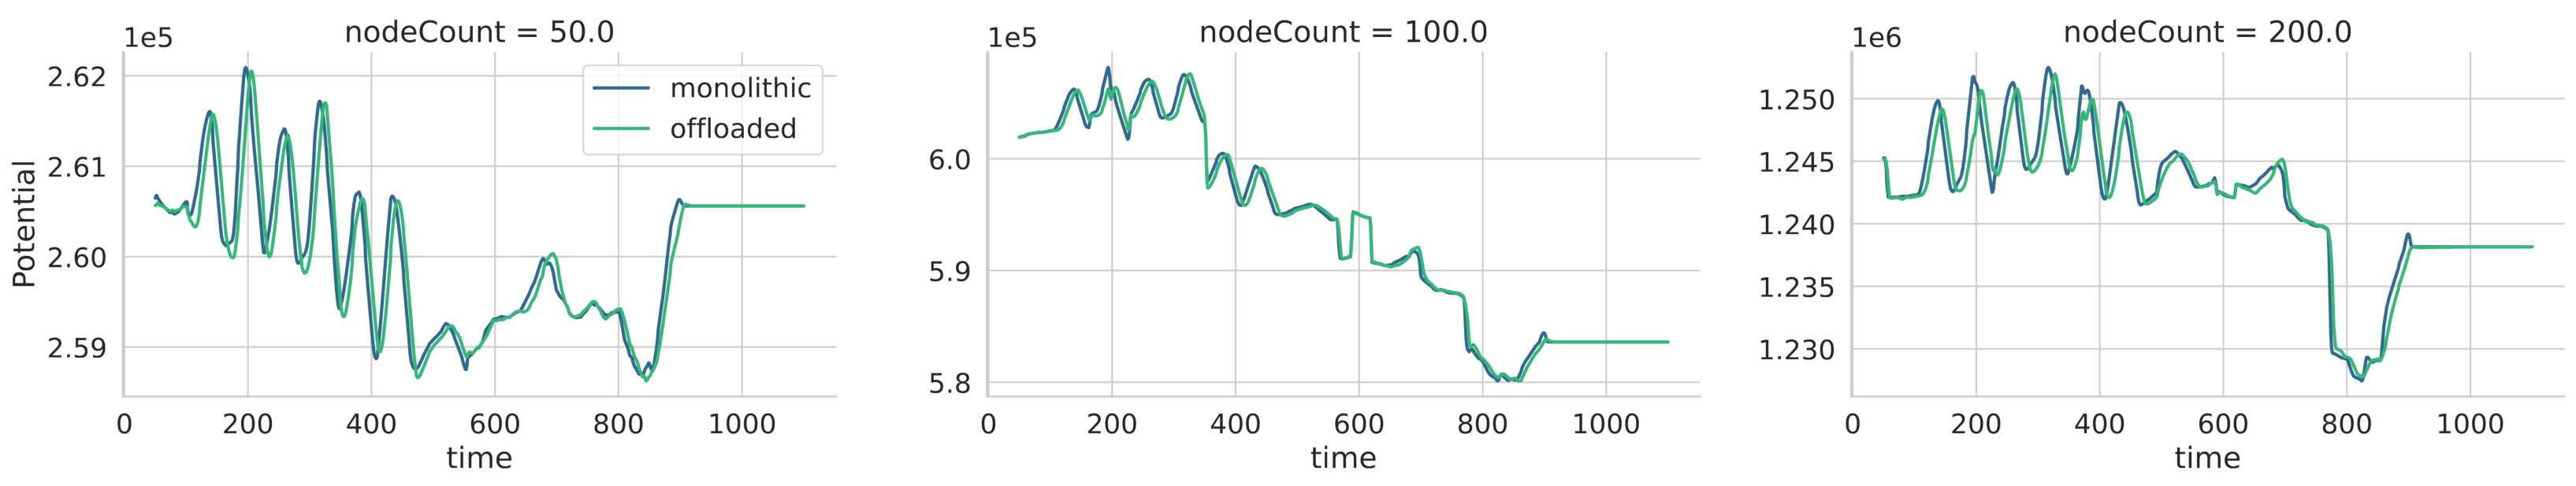
\includegraphics[width=\textwidth]{gradient-convergence.pdf}
    \\[0.4em]
    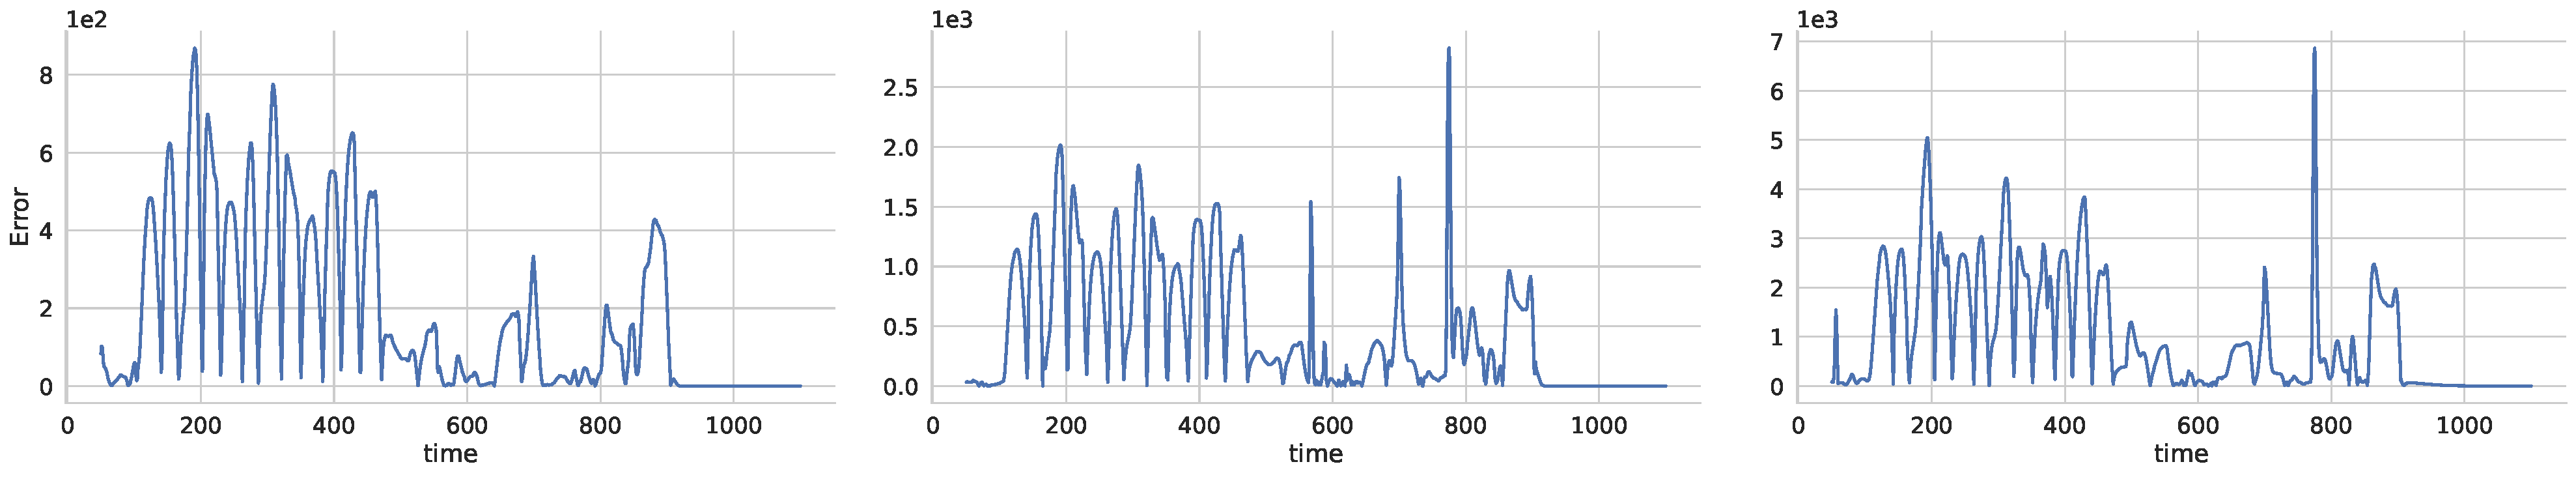
\includegraphics[width=\textwidth]{gradient-convergence-error.pdf}
    \caption[Gradient potential and error between monolithic and offloaded deployments]{Gradient potential under a monolithic and an offloaded deployment, for networks of 50, 100, and 200 nodes (top), and the error between the two deployments over the same runs (bottom). Data from~\cite{DBLP:conf/acsos/FarabegoliVC24}.}
    \label{fig:gradient-convergence}
\end{figure}

\Cref{fig:gradient-convergence} shows the two deployments tracking each other closely while the nodes move,
with the error between them driven by the extra hops forwarding introduces during that transient.
%
Once the nodes stop moving at $t=900$,
the error falls to a small residual and recovers after transient perturbations.

\begin{figure}[t]
    \centering
    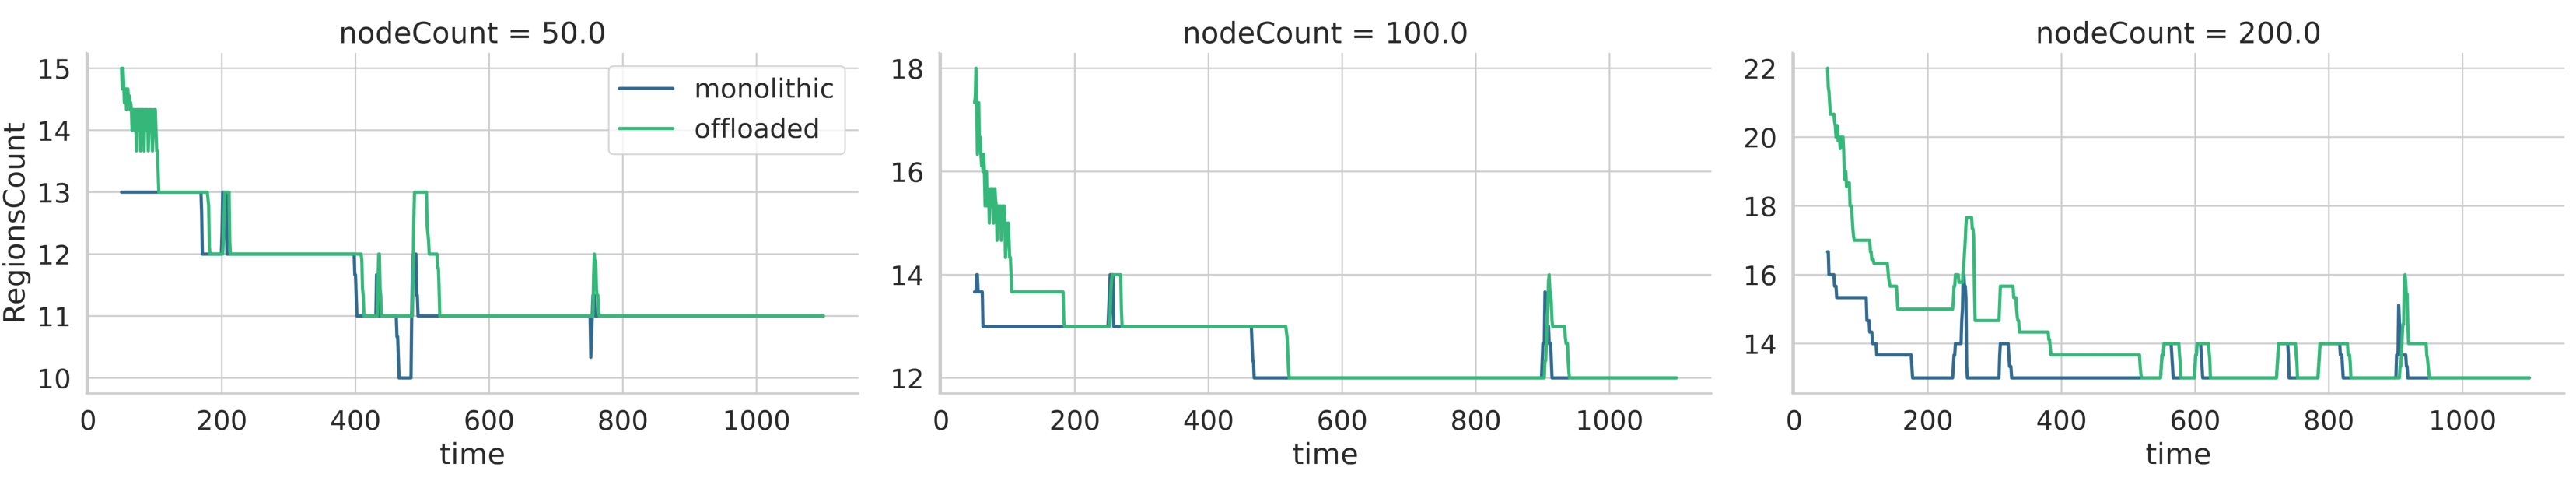
\includegraphics[width=\textwidth]{scr-convergence.pdf}
    \\[0.4em]
    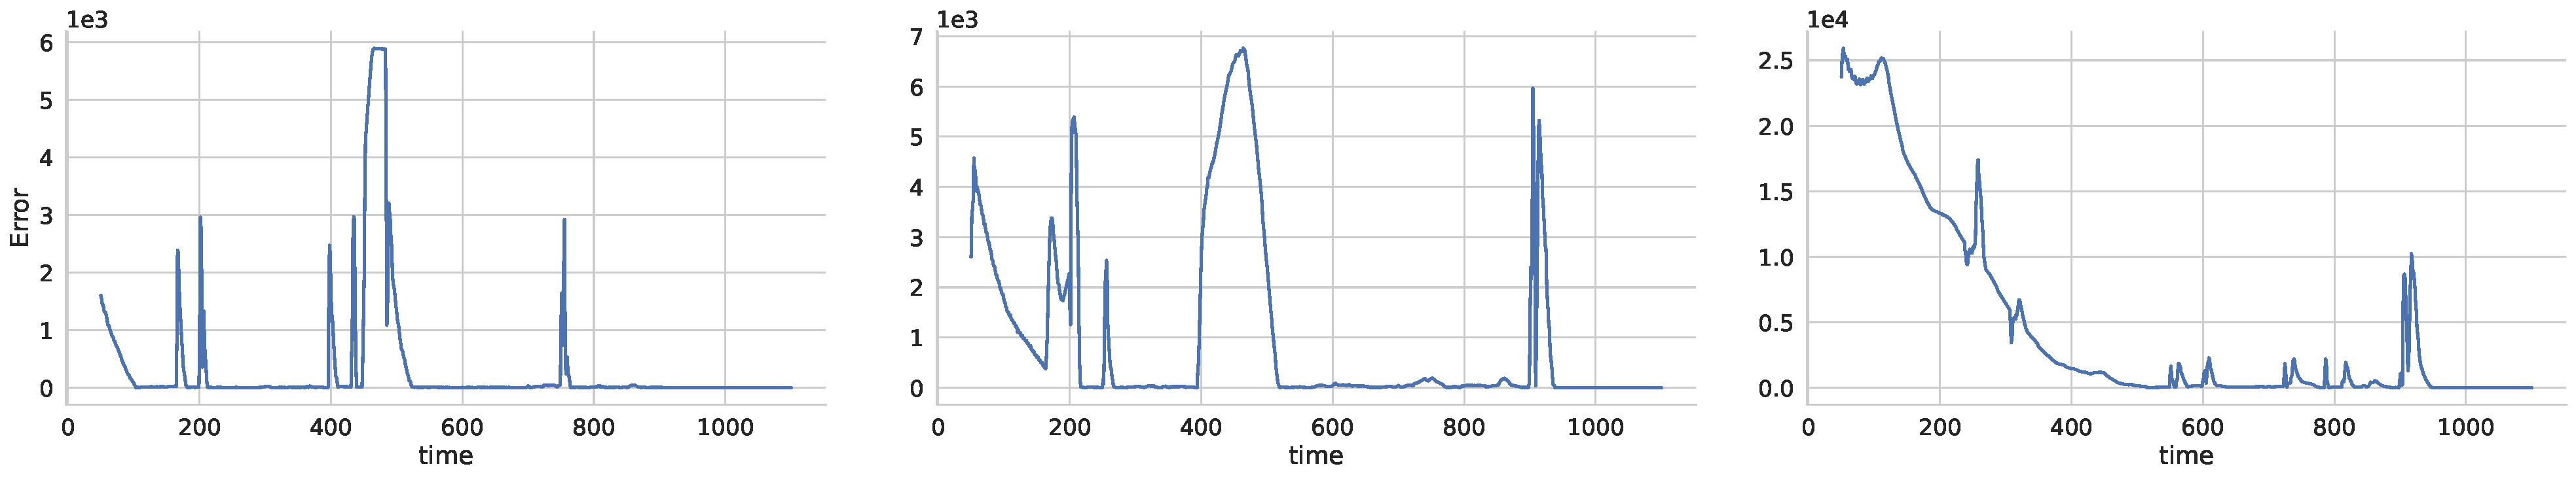
\includegraphics[width=\textwidth]{scr-convergence-error.pdf}
    \caption[Coordination-region count and error between monolithic and offloaded deployments]{Number of self-organising coordination regions the network settles into, under a monolithic and an offloaded deployment (top), and the error between the two (bottom). Data from~\cite{DBLP:conf/acsos/FarabegoliVC24}.}
    \label{fig:scr-convergence}
\end{figure}

\Cref{fig:scr-convergence} repeats the comparison for the region-partitioning service.
%
Larger networks take longer to agree on a stable partition and produce noisier error traces while the topology is still moving,
but every network size drives the offloaded deployment onto the same region count as the monolithic one once movement stops,
regardless of how many components were forwarded and to which surrogate.

\section{Discussion}
\label{sec:pulverization-discussion}

The partitioning developed here and the original five-component one cut along different axes.
Casadei et al.\ divide a logical device by the stages of its execution cycle -- sensing, actuation, behaviour, state, communication -- and obtain the same five deployable units for every application~\cite{DBLP:journals/fi/CasadeiPPVW20}.
This chapter divides a macro-program by its own data flow, and obtains one unit per component of that flow.
The two decompositions can be combined:
a component of the \ac{DAG} is itself a small logical device, with its own sensing, state, and communication concerns,
so the five-role decomposition can be applied inside a component once the data-flow decomposition has fixed what the components are.
Nothing in the model forbids this, and the middleware built for the five-role case already places units of exactly that kind~\cite{DBLP:journals/fgcs/FarabegoliPCV24}.

The model has three limits.
First, component instances are assumed to carry no state beyond what their round-inputs supply,
which is what allows a surrogate to serve many owners as one and a chain to be extended without bookkeeping;
components with private state across rounds fall outside this assumption and would require separate treatment.
Second, \cref{thm:deployment-independence} is a statement about eventual behaviour.
It licenses any correct deployment as functionally equivalent to any other, and says nothing about how fast each converges,
so a deployment chosen on non-functional grounds can still be a poor one on timing grounds.
Third, the deployment is taken as given.
The model says which deployments are admissible and that the choice among them is functionally free;
it does not say how the choice is made, nor who revises it as the infrastructure drifts.


The theorem supports choosing a deployment according to capability, load, or energy requirements,
provided its assumptions remain satisfied.
Convergence time and the costs of communication and reconfiguration still need to be assessed when selecting and revising a deployment.
\clearpage
